\selectlanguage{english}

The Standard Model of Particle Physics (SM) is, as of now, the most complete theoretical framework in subatomic physics, describing all known elementary particles and fundamental interactions \cite{Glashow-1961, Salam-1964, Weinberg-1967, Fritzsch-1972, Fritzsch-1973, Higgs-1964-1, Higgs-1964-2, Englert-1964, Guralnik-1964}, except for the very weak gravitational force. Over the last fifty years, the SM has been continuously tested via numerous experiments, mainly in the context of particle colliders, and its validity has been confirmed by the agreement of its predictions with experimental observations, culminating in 2012 with the discovery of the Higgs boson \cite{ATLAS-2012, CMS-2012} at the Large Hadron Collider (LHC) at CERN.

Despite its success, there is strong evidence for the existence of Physics Beyond the SM (BSM): the most prominent indications include the existence of dark matter and dark energy, the observed matter-antimatter asymmetry and the non-vanishing neutrino masses. Contrary to earlier expectations, though, since its first run in 2009 the LHC has not yet detected any new particle, nor any confirmation of BSM physics: instead, the huge amount of data collected in its three runs (Run 3 is currently ongoing) puts increasingly stricter exclusion limits on BSM models \cite{CMS-ATLAS-SUSY, Bsekidt-2012, Ghosh-2025, Crivellin-2015}. As a consequence, the allowed masses of hypothesized new particles have become so large that it is unlikely that they will be produced at the LHC in sufficient numbers for detailed studies.

Since a substantial further increase in the energy of colliding particles at the LHC (or any other collider) is currently not feasible, the lack of any observation of BSM physics at the LHC has sparked a change in the research paradigm in high-energy particle physics, as it is clear that BSM physics searches based on the idea of detectable resonant-like structures on top of flat backgrounds has to be supplemented by new research strategies. Indeed, new particles can still be produced at the LHC, though in a way which does not allow for their direct detection: undetected light particles could be hidden in complex final states, while heavy particles could be virtually produced for extremely short periods of time, before disappearing back into the quantum vacuum. In the latter case, these virtual particles could affect measurable properties, prompting their indirect detection as deviations from SM predictions.
%
%[ EFT ARGUMENTS ]

Given this shift of focus towards higher experimental precision in collider physics, it is clear that reliable theoretical predictions of hadron-collision processes are needed.

\section{QCD in collider physics}
\label{sec:coll-phys}

In general, any precision study at a hadron collider is challenging to perform, given the poorly-understood nature of the strong force which keeps hadrons together. In fact, the strong interaction is described by Quantum Chromodynamics (QCD), which has the complicated mathematical structure of a non-Abelian gauge theory (\secref{ssec:gauge-th} for details).

Although it has not been possible, so far, to fully describe the properties of a single proton from first principles, in the context of hadron collisions a first-principles description is made possible for a particular class of processes: hard scattering processes, which are characterized by a large momentum transfer.

Even though hard scattering processes have a lower probability of happening, with respect e.g. to elastic scattering processes, they are of great interest to modern particle physics: in fact, these are the processes which produce electroweak (EW) bosons, the Higgs boson, new heavy particles, etc., thus allowing for their detailed study. Moreover, the analysis of hard scattering processes is facilitated by a remarkable property of QCD: \bctxt{asymptotic freedom}.

Asymptotic freedom is a property of certain non-Abelian gauge theories. After the renormalization of a quantum field theory (QFT), the coupling constant of the interaction becomes dependent on a renormalization energy scale, a phenomenon known as the ``running of the coupling" (see \secref{sec:renorm}). The evolution of the running coupling $ \alpha(\mu^2) $ as a function of the energy scale $ \mu $ is described by the renormalization group equation (see e.g. Chapter 12 of \cite{Peskin-1995}):
\begin{equation}
  \mu^2 \frac{\dd \alpha(\mu^2)}{\dd \mu^2} = - 2 \beta(\alpha(\mu^2)) \alpha(\mu^2)
  \label{eq:ren-gr}
\end{equation}
where the Callan--Symanzik $ \beta $-function has a power-series expansion like:
\begin{equation}
  \beta(\alpha) = \sum_{n \in \N_0} \beta_n \left( \frac{\alpha}{4\pi} \right)^{n+1} = \beta_0 \frac{\alpha}{4\pi} + \smo(\alpha^2)
  \label{eq:beta-func}
\end{equation}
For QCD\footnotemark $ \,\beta_0 > 0 $ (see \cite{Gross-1973, Politzer-1973}), hence the coupling becomes small at high energies (small distances). This allows for a perturbative description of hard scattering processes: these events happen at small distances, hence the hadronic scattering can be studied through the interaction between individual partons (see \figref{fig:part-scatt}), i.e. the quarks and gluons which compose the hadrons.

\footnotetext{To be precise, for a $ \SUn{n_c} $ gauge theory with $ n_q < \frac{11}{2} \caa $ active quark flavours, see \secref{ssec:sun}.}

\begin{figure}
  \centering
  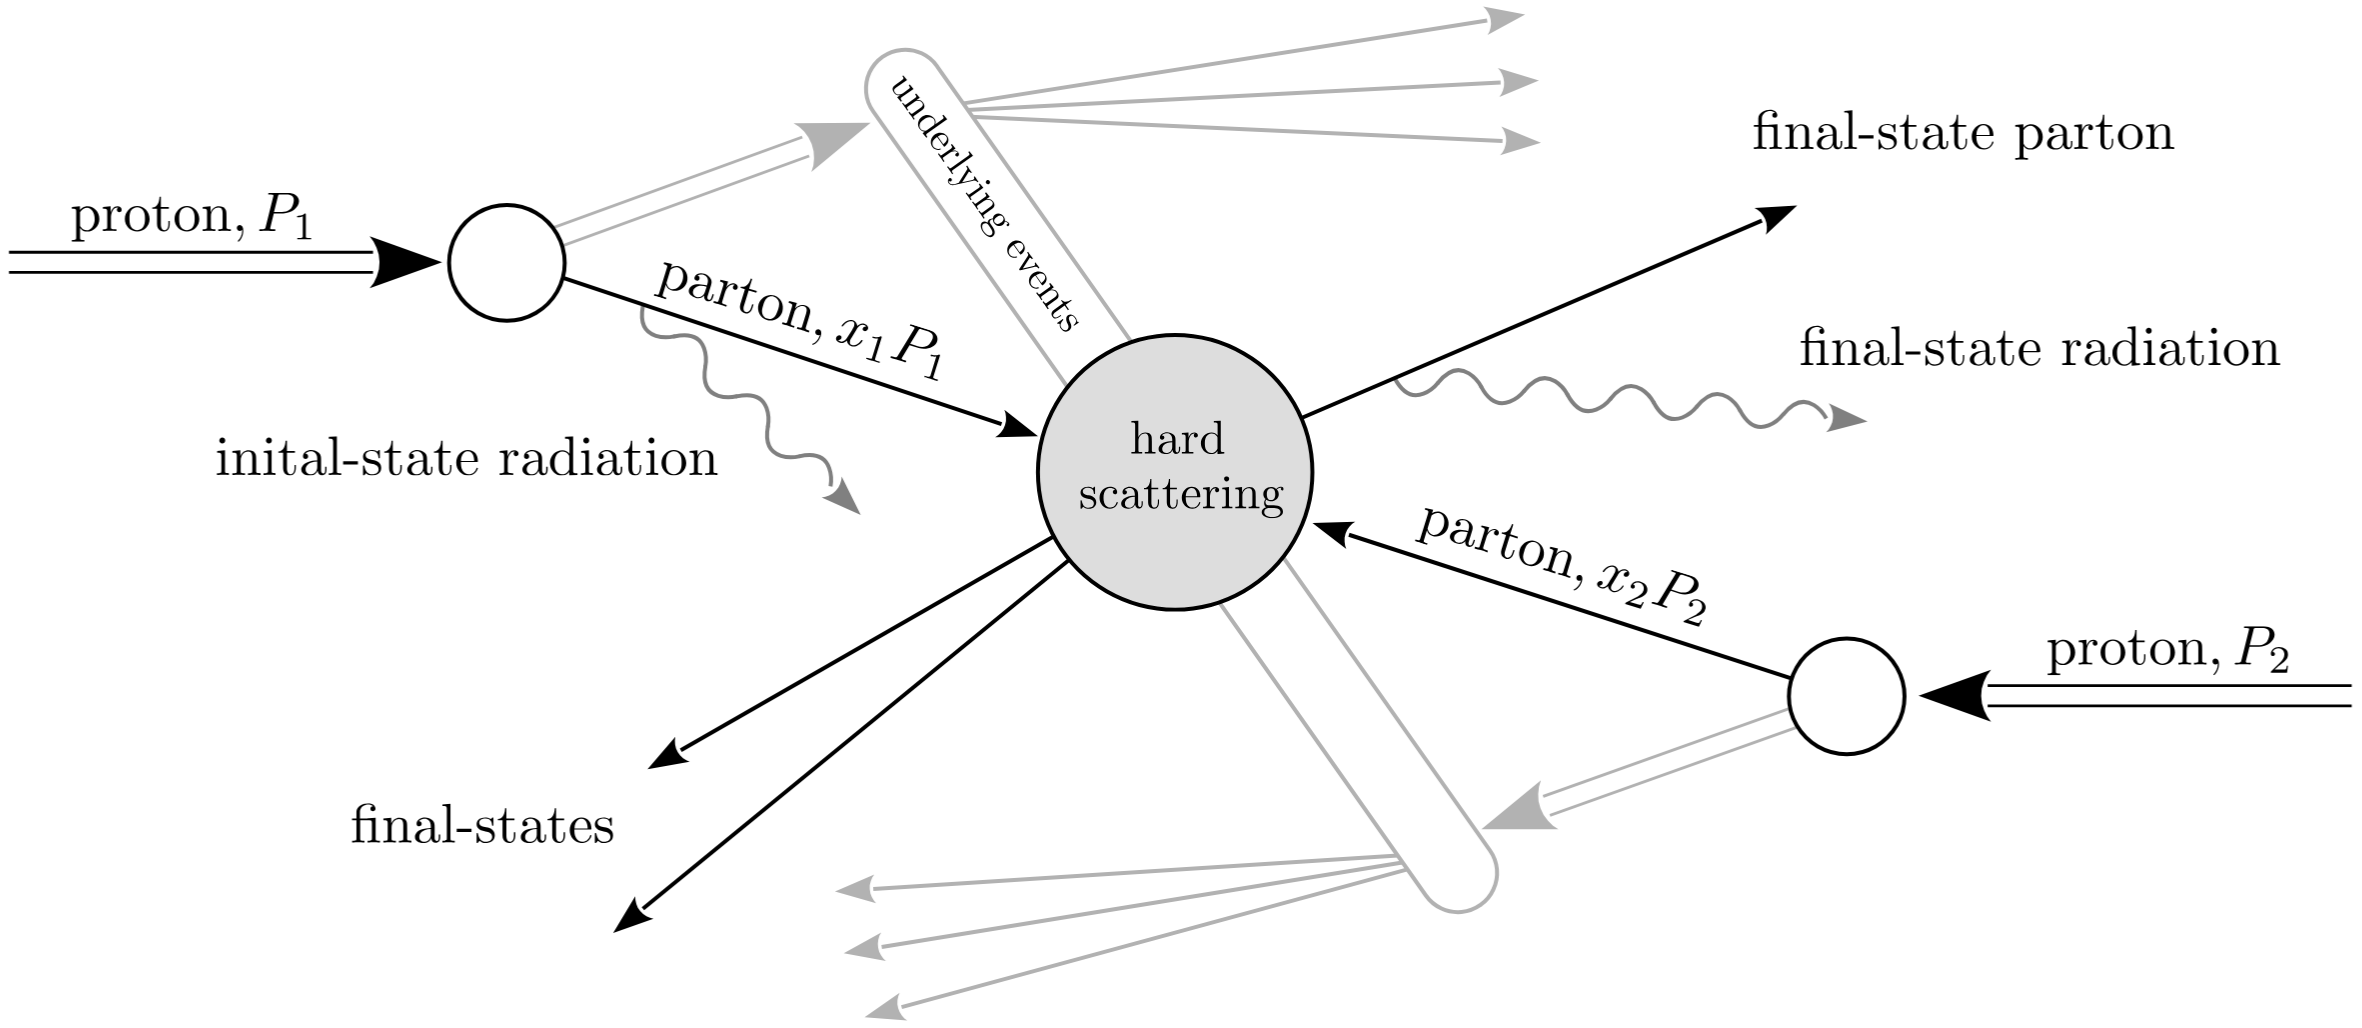
\includegraphics[width = 0.90 \textwidth]{part-scatt.png}
  \caption{Schematics of hard hadronic scattering. Due to asymptotic freedom, individual partons can be assumed to be free particles, so that their (hard) scattering can be computed via perturbative QCD. Initial- and final-state radiation accounts for beyond-leading-order effects. Figure from \cite{Asteriadis-2020}.}
  \label{fig:part-scatt}
\end{figure}

\subsection{Hadronic scattering}

Given the asymptotic freedom of QCD, it is clear why hard scattering processes are preferred for precision studies at hadron colliders: these scatterings occur at high energy $ Q \sim 100\gev - 1\tev $ (at the LHC), hence non-perturbative effects are suppressed by powers of $ \qcd / Q $, where $ \qcd \approx 200\mev $ is an energy scale describing the asymptotic freedom of QCD (see below). This is formalized by the factorization theorem \cite{Collins-1989}, which states that hadronic cross-sections can be computed from partonic cross-sections as:
\begin{multline}
  \dd\hcs_{h_1,h_2}(P_1 , P_2) = \sum_{a,b} \int_{[0,1]^2} \frac{\dd \xi_1}{\xi_1} \frac{\dd \xi_2}{\xi_2} \, \pdfb{a}{h_1}(\xi_1, \fac^2) \pdfb{b}{h_2}(\xi_2, \fac^2) \times \\
  \times \dd\pcs_{a,b}(\xi_1 P_1, \xi_2 P_2, \rc, \ren^2, \fac^2)
  \left[ 1 + \smo \left( \frac{\qcd^n}{Q^n} \right) \right]
  \label{eq:fact-th}
\end{multline}
with $ n \in \N $. Here, the two scattering hadrons $ h_1 , h_2 $ have momenta $ P_1 , P_2 $, while the scattering partons $ a , b $ have momentum fractions $ \xi_1 , \xi_2 $. For the rest of this work, the factorization scale $ \fac $ is taken to be equal to the renormalization scale $ \ren $ defined in \secref{ssec:min-sub}. Finally, $ \dd\pcs_{a,b} $ is the partonic cross-section to be discussed in the next subsection.

The link between hadron-scale physics and parton-scale physics is given by \bctxt{parton distribution functions} (PDFs): in general, $ \pdfb{a}{h}(\xi) $ is the numerical probability of finding a parton $ a $ inside the hadron $ h $ with a definite momentum fraction $ \xi : p_a = \xi P_h $, where $ p_a $ and $ P_h $ are the momenta of the parton and of the hadron, respectively. A crucial property of PDFs is their universality, as they are process-independent: this means that they can be measured in a particular process and then used in many others. However, they encapsulate non-perturbative effects which are poorly understood, thus they have not been computed from first principles so far.

Another instance of non-perturbative effects arises when considering that, after the partonic interaction, final-state partons can be clustered into so-called jets: despite the difficulty in formally defining jets (for a review of various jet algorithms, see \cite{Salam-2010}), they can be intuitively pictured as seeds of hadronic energy flows which are barely affected by non-perturbative QCD effects. However, while on short time-scales QCD can be treated perturbatively, on long time-scales QCD partons (and so jets too) are subject to the phenomenon of \bctxt{hadronization}. Hadronization can be explained by considering a solution to \eref{eq:ren-gr} at leading-order in $ \alpha $, found by introducing a reference scale $ \mu $:
\begin{equation}
  \rcr = \frac{\rc(\mu^2)}{1 + 2 \rc(\mu^2) \frac{\beta_0}{4\pi} \log \frac{\ren^2}{\mu^2}}
\end{equation}
For example, $ \rc(m_Z^2) \approx 0.118 $ \cite{PDG-2024}. It is customary to introduce a QCD scale $ \qcd $, defined as (see Chapter 2 of \cite{Ellis-1996}):
\begin{equation}
  \ln \frac{\ren^2}{\qcd^2} \equiv \frac{1}{2} \int_{\rcr}^\infty \frac{\dd x}{x \beta(x)}
\end{equation}
Experimental analysis sets $ \qcd \approx 200\mev $. Retaining only the $ \beta_0 $ term allows expressing the running coupling as:
\begin{equation}
  \rcr \equiv \frac{1}{2\frac{\beta_0}{4\pi} \log \frac{\ren^2}{\qcd^2}}
\end{equation}
This expression shows that $ \ren \gg \qcd $ is the perturbative region, where asymptotic freedom makes $ \rc $ small enough for perturbative techniques. On the other hand, for $ \ren \rightarrow \qcd $ a Landau pole is present: this pole signals the breakdown of perturbation theory and the hadronization of partons, i.e. their confinement into bound states (hadrons).

\begin{figure}
  \centering
  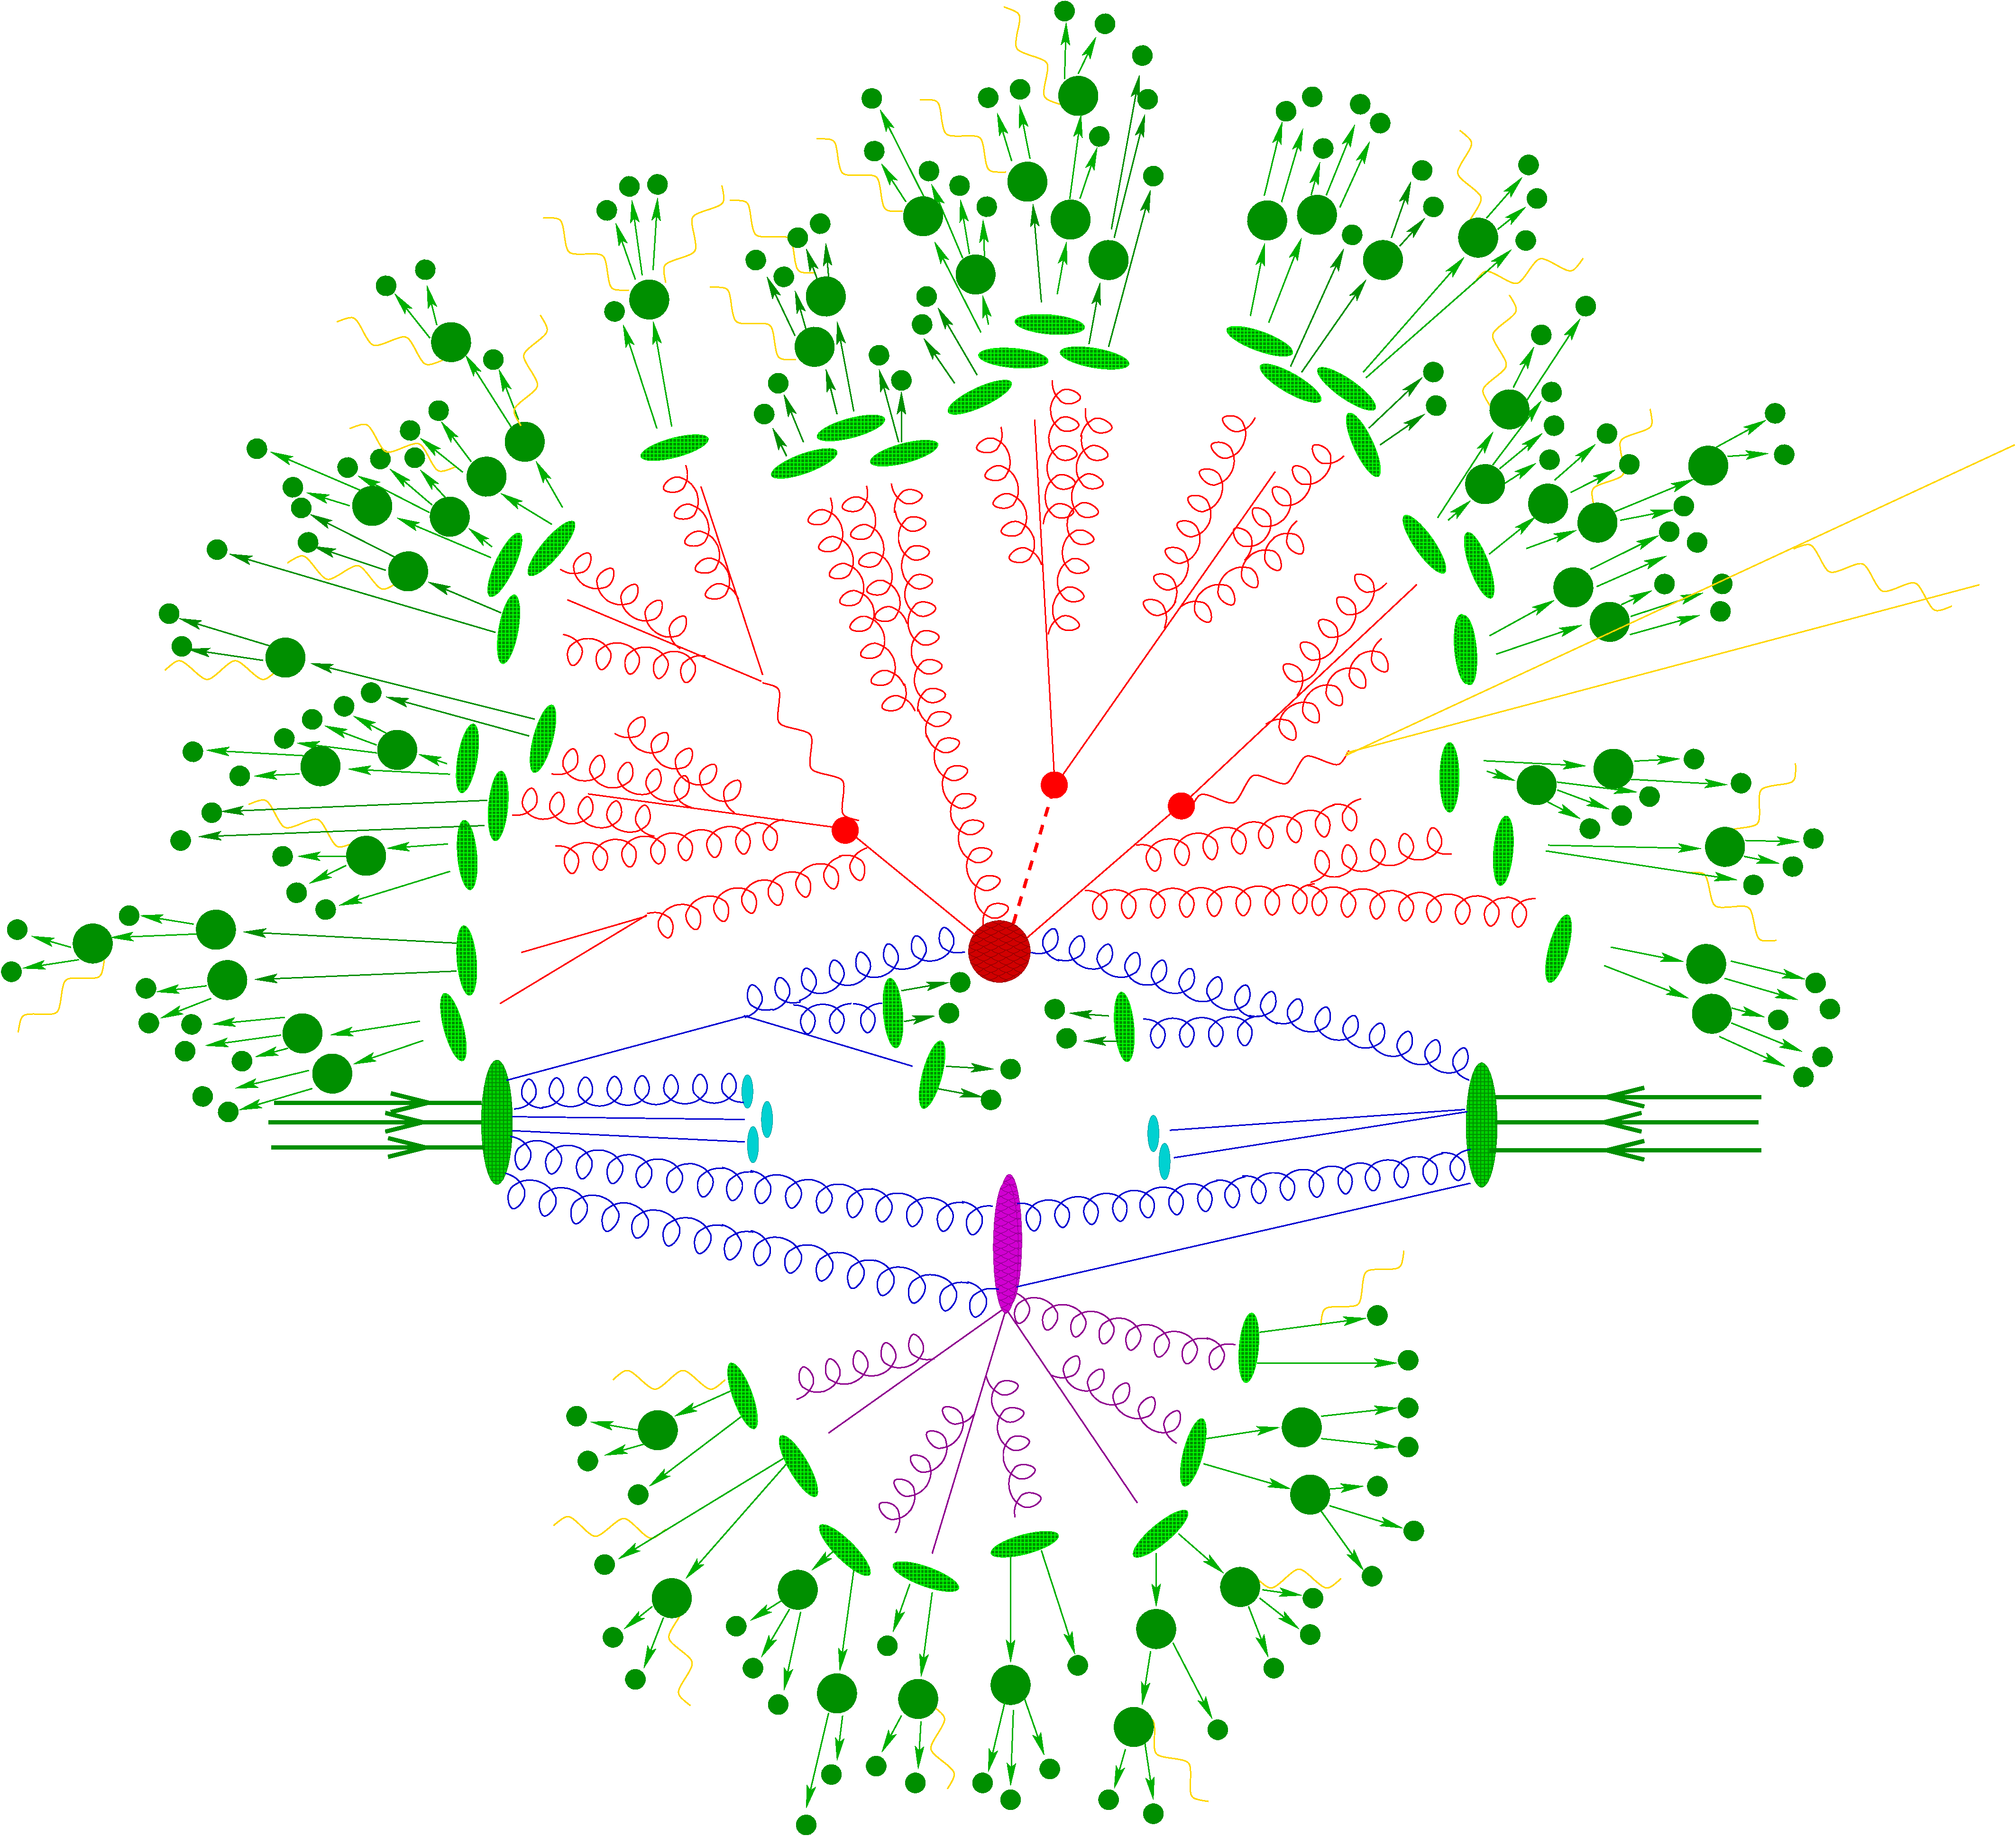
\includegraphics[width = 1.00 \textwidth]{hadr-scatt.pdf}
  \caption{Hadronization of jets produced in a hard hadronic scattering. Incoming hadrons produce incoming partons (blue) which, after emitting some initial-state radiation, enter the hard scattering event (red blobs) as well as a double parton scattering (purple blob, not considered in this work): these scatterings give rise to partonic jets (red and purple) which undergo hadronization (light green blobs), eventually forming heavy hadrons (dark green blobs) and producing soft radiation (yellow). Figure from \cite{Hoche-2014}.}
  \label{fig:hadr-scatt}
\end{figure}

\eref{eq:fact-th} can be represented graphically as in \figref{fig:hadr-scatt}. Here, the hard scattering process occurs at high energy $ Q \gg \qcd $, resulting in jets which are initially unaffected by non-perturbative QCD, since their energy is well above the QCD scale; however, this energy is radiated off in the form of parton showers, and, when the threshold energy $ \qcd $ is reached, non-perturbative effects come into play, resulting in the hadronization of jets.

The factorization theorem also provides a numerical estimate for corrections due to non-perturbative effects. Setting the lowest energy scale of the considered scattering (e.g. a $ \tm $-cut on a jet) to be $ Q \approx 20\gev $ and $ n = 1 $ in \eref{eq:fact-th}, then non-perturbative corrections are of order $ \sim 10^{-2} $, i.e. percentage-level corrections.

\subsection{Partonic scattering}

For the rest of this work, the analysis is restricted to partonic scattering treated using perturbation theory. Thus, the partonic cross-section for the scattering of two partons $ a , b $ with momenta $ p_1 , p_2 $ can be expressed as a power series in the running coupling:
\begin{equation}
  \dd\pcs_{a,b}(p_1 , p_2) = \sum_{n \in \N_0} \dd\pcs_{a,b}^{(n)}(p_1 , p_2)
  \label{eq:part-ser-exp}
\end{equation}
where each term is $ \dd\pcs^{(n)} \sim \rc^{n_0 + n} $, with $ n_0 \in \N $ giving the dependence on $ \rcr $ due to the leading-order (LO) process, which is usually (but not always) a tree-level process.

The $ n \ge 1 $ terms are referred to as QCD corrections. Focusing on next-to-leading-order (NLO) corrections, they can be of two kinds: real corrections and virtual corrections. Real corrections consist in the emission of an additional parton as initial- or final-state radiation, while virtual corrections present an additional partonic loop. Examples of a real and a virtual correction to the Drell-Yan process may be:
\begin{equation*}
  \begin{tikzpicture}
    \begin{feynman}

      \vertex (a1) {\(q\)};
      \vertex[below = 3cm of a1] (a2) {\(\bar{q}\)};

      \vertex[below = 1.5cm of a1] (b1) {};
      \vertex[right = 2.25cm of b1, dot] (v1) {};

      \vertex[right = 2.25cm of v1, dot] (v2) {};
      \vertex[right = 2.25cm of v2] (b2) {};

      \vertex[above = 1.5cm of b2] (a3) {\(e^-\)};
      \vertex[below = 1.5cm of b2] (a4) {\(e^+\)};

      \vertex[dot] (c1) at ($(a1) + (1.5,-1)$) {};
      \vertex (c2) at ($(c1) + (1.5,1)$) {\(g\)};

      \diagram* {
	(a1) -- [fermion] (v1),
	(a2) -- [anti fermion] (v1),

	(v1) -- [photon, edge label = \(\gamma^*\)] (v2),

	(v2) -- [fermion] (a3),
	(v2) -- [anti fermion] (a4),

	(c1) -- [gluon] (c2),
      };
    \end{feynman}
  \end{tikzpicture}
  \qquad \qquad
  \begin{tikzpicture}
    \begin{feynman}

      \vertex (a1) {\(q\)};
      \vertex[below = 3cm of a1] (a2) {\(\bar{q}\)};

      \vertex[below = 1.5cm of a1] (b1) {};
      \vertex[right = 2.25cm of b1, dot] (v1) {};

      \vertex[right = 2.25cm of v1, dot] (v2) {};
      \vertex[right = 2.25cm of v2] (b2) {};

      \vertex[above = 1.5cm of b2] (a3) {\(e^-\)};
      \vertex[below = 1.5cm of b2] (a4) {\(e^+\)};

      \vertex[dot] (c1) at ($(a1) + (0.75,-0.5)$) {};
      \vertex[dot] (c2) at ($(a2) + (0.75,0.5)$) {};

      \diagram* {
	(a1) -- [fermion] (v1),
	(a2) -- [anti fermion] (v1),

	(v1) -- [photon, edge label = \(\gamma^*\)] (v2),

	(v2) -- [fermion] (a3),
	(v2) -- [anti fermion] (a4),

	(c1) -- [gluon, bend right, edge label' = \(g^*\)] (c2),
      };
    \end{feynman}
  \end{tikzpicture}
\end{equation*}
In general, then:
\begin{equation}
  \dd\pcs_{a,b}^{(1)}(p_1 , p_2) = \dd\pcsr_{a,b}(p_1 , p_2) + \dd\pcsv_{a,b}(p_1 , p_2) + \dd\pcspdf_{a,b}(p_1 , p_2)
  \label{eq:real-exp}
\end{equation}
where $ \dd\pcsr_{a,b} $ and $ \dd\pcsv_{a,b} $ are the single-real and one-loop corrections. The additional correction $ \dd\pcspdf_{a,b} $ is due to the collinear renormalization of PDFs.

\section{Singularities in QCD amplitudes}
\label{sec:sing}

One of the main difficulties when computing real and virtual corrections to scattering amplitudes is the presence of singularities in particular kinematic limits.

\subsection{Infrared poles}
\label{ssec:ir-poles}

In the case of amplitudes with real emissions, singularities arise when the energy of a gluon vanishes (\bctxt{soft singularity}) or when two massless partons are emitted in the same direction (\bctxt{collinear singularity}). To illustrate why the amplitude diverges in these limits, consider a real-emission diagram like:
\begin{equation*}
  \begin{tikzpicture}[baseline = (r.base)]
    \begin{feynman}[inline = (r.base)]
      \vertex (a);
      \vertex[right = 2.5cm of a, dot] (b) {};
      \vertex[right = 2.5cm of b, blob, minimum size = 1.2cm] (c) {};

      \vertex[above = 1.5cm of b] (d);
      \vertex[right = 1.5cm of d] (e);

      \vertex[below = 0.25em of b] (r);

      \diagram* {
	(a) -- [fermion, momentum' = \(p\)] (b),
	(b) -- [fermion, momentum' = \(p - k\)] (c),

	(b) -- [gluon, momentum = \(k\)] (e),
      };
    \end{feynman}
  \end{tikzpicture}
  \quad \sim \quad
  \frac{1}{(p - k)^2} = - \frac{1}{2 E_p E_k \left( 1 - \cos \theta \right)}
\end{equation*}
where the massless approximation\footnotemark for the quark is employed. It is then clear that the amplitude diverges for $ E_k \rightarrow 0 $ and $ \theta \rightarrow 0 $ due to the propagator of the virtual quark; note that single quark emissions do not give rise to any soft singularities, as in the massless limit they provide an integrable singularity (due to the presence in the matrix element of spinors $ u^s(p) \sim \sqrt{E_p} $).

\footnotetext{In the context of collider physics, light quarks are usually approximated as massless, as they have $ m_q / Q \lesssim 10^{-3} $, with $ Q \sim 100\gev - 1\tev $ in a typical LHC process. The only exceptions are the heavy flavours: the bottom quark is sometimes treated as massive ($ m_b \approx 4.18 \gev $), while the top quark is always treated as massive ($ m_t \approx 172 \gev $). Data from \cite{PDG-2024}.}

Both kinds of singularities in real emissions can be seen as one virtual massless parton going on-shell (in the above example, the virtual quark with momentum $ q = p - k $ in the massless approximation), i.e. with $ q^2 \rightarrow 0 $, and they are collectively called infrared-collinear singularities, or commonly (though less precisely) infrared (IR) singularities.

It is important to note that massive partons do not determine soft or collinear singularities, as shown e.g. by $ g \rightarrow q + \bar{q} $ splitting:
\begin{equation*}
  \begin{tikzpicture}[baseline = (r.base)]
    \begin{feynman}[inline = (r.base)]
      \vertex (a);
      \vertex[right = 2.5cm of a, dot] (b) {};
      \vertex[right = 2.5cm of b, blob, minimum size = 1.2cm] (c) {};

      \vertex[above = 1.5cm of b] (d);
      \vertex[right = 1.5cm of d] (e);

      \vertex[below = 0.25em of b] (r);

      \diagram* {
	(a) -- [gluon, momentum' = \(p\)] (b),
	(b) -- [anti fermion, momentum' = \(p - k\)] (c),

	(b) -- [fermion, momentum = \(k\)] (e),
      };
    \end{feynman}
  \end{tikzpicture}
  \quad \sim \quad
  \frac{1}{(p - k)^2 - m^2} = - \frac{1}{2 E_p \left( E_k - \abs{\ve{k}} \cos \theta \right)}
\end{equation*}
Obviously there is no soft limit in this case, as $ E_k \ge m > 0 $. Moreover, as $ E_k \neq \abs{\ve{k}} $ for $ m > 0 $, the collinear limit $ \theta \rightarrow 0 $ does not produce a singularity.

The case of virtual corrections is more complex. Indeed, virtual-correction amplitudes present an additional loop integral, which has two kinds of singularities: ultraviolent (UV) singularities and IR ones. To illustrate them, consider the following loop diagram:
\begin{equation*}
  \begin{tikzpicture}[baseline = (r.base)]
    \begin{feynman}[inline = (r.base)]

      \vertex (a) {};
      \vertex[right = 2cm of a, dot] (b) {};
      \vertex[right = 2.5cm of b, dot] (c) {};
      \vertex[right = 2cm of c, blob, minimum size = 1.2cm] (d) {};

      \vertex[below = 0.25em of a] (r) {};

      \diagram* {
	(a) -- [gluon] (b) -- [gluon, momentum' = \(p + k\)] (c) -- [gluon] (d),
	(c) -- [gluon, out = 90, in = 90, looseness = 1.5, momentum = \(k\)] (b),
      };
    \end{feynman}
  \end{tikzpicture}
  \quad \sim \quad
  \int \frac{\dd^4k}{(2\pi)^4} \frac{1}{k^2} \frac{1}{(p + k)^2}
\end{equation*}
The UV divergence can be seen performing a Wick rotation $ k^0 \mapsto i k^0 $ and introducing a cutoff $ \Lambda $ for the Euclidean momentum's magnitude $ \abs{k_\text{E}} $: in the UV limit $ k^2 \gg p^2 $, so the integral is $ \sim \log \Lambda $, which is clearly divergent for $ \Lambda \rightarrow \infty $. However, this kind of divergences is cured through the procedure of renormalization (\secref{sec:renorm}).

IR divergences, on the other hand, have the same origin as those in real corrections: in reality, Nature does not distinguish between ``real" and ``virtual" corrections, which are merely human-made categories introduced to simplify the calculations. To confirm this, while real and virtual corrections present IR divergences when considered individually, these poles have to cancel when the two sets of corrections are added together: this is an instance of the Kinoshita--Lee--Nauenberg theorem, which asserts that the SM is IR-finite \cite{Kinoshita-1962, Lee-1964}.

\subsection{Subtraction method}

The central problem of showing the pole cancellation is the fact that real and virtual corrections have different particle multiplicity in the phase space, so their summation is not straightforward. However, Catani's formula \cite{Catani-1998} allows one to extract IR singularities from renormalized virtual-correction amplitudes as poles in the number of spacetime dimensions (see \secref{ssec:dim-reg}). Luckily, the same can be done with real corrections too: in the IR limits a parton goes unresolved, so the effective phase space has the same multiplicity as that of virtual corrections (see \secref{sec:nsc-real}).

The crucial point of extracting divergences, and in particular from real corrections, is to do so without integrating over the resolved phase space, in order to obtain an expression for the fully-differential (with respect to resolved partons) cross-section which allows for the numerical evaluation of phase-space integrals for any IR-safe observable. To do so, it is necessary to introduce a subtraction method.

To illustrate the idea of a subtraction method, consider the following integral:
\begin{equation}
  I = \int_0^1 \frac{\dd x}{x^{1 + \epsilon}} f(x)
\end{equation}
where $ f(x) $ is an arbitrary integrable function regular at $ x = 0 $. The integrand clearly diverges at $ x = 0 $, and this singularity is regulated by the parameter $ \epsilon $ which leads to a $ \frac{1}{\epsilon} $ pole after integration. The aim of the subtraction method is to analytically extract this pole and regulate the integral, making it finite in the $ \epsilon \rightarrow 0 $ limit. The basic idea is to introduce a counterterm by writing $ f(x) = [f(x) - f(0)] + f(0) $, so that:
\begin{equation*}
  I = \int_0^1 \frac{\dd x}{x^{1 + \epsilon}} \left[ f(x) - f(0) \right] + f(0) \int_0^1 \frac{\dd x}{x^{1 + \epsilon}}
\end{equation*}
The second integral is analytically determined for $ \Re{\epsilon} < 0 $, hence:
\begin{equation}
  I = \int_0^1 \frac{\dd x}{x^{1 + \epsilon}} \left[ f(x) - f(0) \right] - \frac{f(0)}{\epsilon}
  \label{eq:reg-i}
\end{equation}
The pole has successfully been isolated, and the integral is now regular at $ x = 0 $, allowing for its numerical integration after setting $ \epsilon \rightarrow 0 $.

In a similar fashion, subtraction schemes allow for the extraction of IR singularities from QCD corrections. The main challenge is to define $ f(0) $ such that it locally removes all divergences in the first term of \eref{eq:reg-i}, while also allowing the analytic integration of the second term, in a process-independent way. At NLO this problem has been completely solved in a fully-local and analytic way with the Catani--Seymour (CS) scheme \cite{Catani-1997} and the Frixione--Kunszt--Signer (FKS) scheme \cite{Frixione-1996, Frixione-1997}. At NNLO a completely general, analytic and fully-local subtraction scheme has not yet been developed, but there are several candidates: in this work we consider the Nested Soft-Collinear (NSC) subtraction scheme (SS), introduced in \cite{rontsch-2017}.

The NSC SS can be applied to any scattering process with a generic number of final-state massless partons \cite{rontsch-2509}; however, it cannot yet describe processes with final-state massive partons, e.g. top quarks. This work takes the first step in this direction, generalizing the NLO subtraction operators defined in \cite{rontsch-2023, rontsch-2503, rontsch-2509} to account for both massless and massive final-state partons. We first give a general discussion on QCD in chapter 2, focusing on the renormalization scheme used and the colour-space formalism for the amplitudes. Then, we provide an overview of the NSC SS in chapter 3, before extending it to include massive final-state partons in chapter 4. Finally, we conclude in chapter 5 with possible future developments.











